\documentclass[../main.tex]{subfiles}

\begin{document}

\section{Higgs boson}%
\label{sec:higgs_boson}

\subsection{De noot voor een scalair boson}%
\label{sub:de_noot_voor_een_scalair_boson}

Bekijken we de cross secties van een aantal zelf interacties die kunnen plaatsvinden voor de zwakke interactie bosonen dan zien we bij ongeveer 1TeV dat de unitariteit geschonden wordt, de waarschijnlijkheden voor deze diagrammen worden groter dan 1.

\begin{figure}[h]
    \centering
    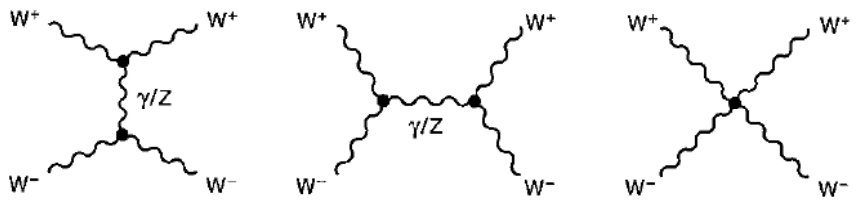
\includegraphics[width=0.8\linewidth]{higgs_boson/zwak_zelf_int_geen_H.png}
    \caption{Mogelijke zelf interactie diagrammen voor het toevoegen van Higgs interacties}%
    \label{fig:higgs_boson/zwak_zelf_int_geen_H}
\end{figure}

Om deze divergenties op te lossen is het nodig om extra parameters toe te voegen. Door het toevoegen van de de koppeling van de $W$ bosonen aan het Higgs boson, een scalair boson, is het mogelijk om de divergentie naar oneindig te convergeren.

\begin{figure}[h]
    \centering
    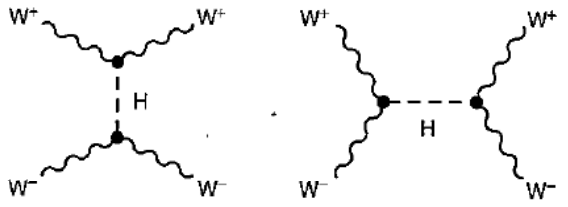
\includegraphics[width=0.6\linewidth]{higgs_boson/zwak_zelf_int_H.png}
    \caption{Toevoegen van Higgs boson interacties}%
    \label{fig:higgs_boson/zwak_zelf_int_H}
\end{figure}

We kunnen aan deze diagrammen direct zien dat de elektrozwakke koppeling van $W$ aan $Z$ een grote invloed zal hebben voor de koppeling van $W$ aan $H$. De opheffing van de divergenties zal enkel werken als de $H$-koppeling gerelateerd is aan de elektrozwakke koppeling.

\subsection{Lagrangiaan}%
\label{sub:lagrangiaan}

Hier moeten we overstappen van het relativistische beeld naar de kwantumvelden theorie omdat Higgs mechanisme en het bestaan van het Higgs boson niet uitgelegd kan worden zonder deze theorie.\\
Klassiek gezien is de Lagrangiaan niets meer dan $L(q_i, \dot{q}_i) = T-V$. Hierbij hoort de klassieke bewegingsvergelijking
\begin{equation}
    \begin{aligned}
        \label{eq:klas_bewegingsvergelijking}
        \frac{d}{dt} \left( \frac{\partial L}{\partial \dot{q}_i} \right) - \frac{\partial L}{\partial q_i} =0
    \end{aligned}
\end{equation}
Wanneer we overschakelen naar veldentheorie worden de plaats en impuls componenten vervangen door veldcoordinaten en zijn afgeleiden, $L(q_i,\dot{q}_i) \rightarrow \mathcal{L}(\phi_i, \partial_\mu\phi_i)$. De bewegingsvergelijking voor de veldentheorie is in essentie gelijk aan de klassieke bewegingsvergelijking.
\begin{equation}
    \begin{aligned}
        \label{eq:velden_bewegingsvergelijking}
        \partial_\mu \left( \frac{\partial \mathcal{L}}{\partial(\partial_\mu \phi_i)} \right) - \frac{\partial \mathcal{L}}{\partial \phi_i} = 0
    \end{aligned}
\end{equation}
In de quantumvelden theorie zijn de deeltjes niet meer dan de kleinste excitaties van de velden, de kwanta. De Lagrangiaan kan nu op verschillende manieren samengesteld worden om verschillende deeltjes te beschrijven. Een aantal voorbeelden hiervan zijn:
\begin{itemize}
    \item Scalair: Deze deeltjes dragen geen spin en pariteit en worden beschreven door
        \begin{equation}
            \begin{aligned}
                \label{eq:lagr_scalair}
                \mathcal{L}_S = \frac{1}{2} (\partial_\mu \phi)(\partial^\mu \phi) = \frac{1}{2} m^2\phi^2
            \end{aligned}
        \end{equation}
        De veldfuncties $\phi$ die door deze Lagrangiaan beschreven worden voldoen aan de Klein-Gordon vergelijkingen. De kwanta hiervan zijn Higgs bosonen.
    \item Dirac: Dirac deeltjes worden beschreven door
        \begin{equation}
            \begin{aligned}
                \label{eq:lagr_dirac}
                \mathcal{L}_D = i\overline \psi \gamma^\mu \partial_\mu \psi - m \overline \psi\psi
            \end{aligned}
        \end{equation}
        De veldgolffuncties voldoen hier natuurlijk aan de Dirac vergelijking en zijn dus 4 vectoren met als kwanta de fermionen.
        \begin{equation}
            \begin{aligned}
                \label{eq:veld_func_dirac}
                \psi(x) =
                \begin{pmatrix}
                    \psi_1\\
                    \psi_2\\
                    \psi_3\\
                    \psi_4\\
                \end{pmatrix}=
                \begin{pmatrix}
                    \Psi_1 + i\Phi_1\\
                    \Psi_2 + i\Phi_2\\
                    \Psi_3 + i\Phi_3\\
                    \Psi_4 + i\Phi_4\\
                \end{pmatrix}
            \end{aligned}
        \end{equation}
    \item Vector: Ten laatste wordt de vector Lagrangiaan gegeven door
        \begin{equation}
            \begin{aligned}
                \label{eq:lagr_vec}
                \mathcal{L}_{EM} = - \frac{1}{4} F^{\mu\nu}F_{\mu\nu}
            \end{aligned}
        \end{equation}
        Deze veldfuncties $F_{\mu\nu}$ volgen de Maxwell vergelijkingen en kunnen neergescheven worden als
        \begin{equation}
            \begin{aligned}
                \label{eq:veld_func_em}
                f^{\mu\nu} = \partial^\mu A^\nu - \partial^\nu A^\mu =
                \begin{pmatrix}
                    0 & -E_x & -E_y & -E_z \\
                    E_x & 0 & -B_z & B_y \\
                    E_y & B_z & 0 -B_x \\
                    E_z & -B_y & B_x & 0 \\
                \end{pmatrix}
            \end{aligned}
        \end{equation}
        De kwanta van dit veld zijn fotonen.
\end{itemize}

\subsection{Lakale $U(1)$ ijk(=gauge) invariantie}%
\label{sub:lakale_u_1_gauge_invariantie}

Als we eisen dat de Lagrangiaan invariant moet zijn onder $\psi(x) \rightarrow \psi'(x) = e^{iq\chi(x)}\psi(x)$. Dit is niets anders dan de fase overal te gaan veranderen of dit kan ook gezien worden als een rotatie in de ruimte met hoek $\chi(x)$. De ruimte afhankelijkheid van de hoek slaat neet op het lokale gedeelte van de invariantie. Bijvoorbeeld voor de Dirac Lagrangiaan krijgen we dan
\begin{equation}
    \begin{aligned}
        \label{eq:lok_ijk_inv_dir_1}
        \mathcal{L} &= i\overline \psi \gamma^\mu \partial_\mu \psi - m \overline \psi\psi\\
        \mathcal{L} \rightarrow \mathcal{L}' &= i e^{-iq\chi} \overline \psi \gamma^\mu [e^{iq\chi}\partial_\mu \psi + iq(\partial_\mu\chi) e^{iq\chi}\psi] - m e^{iq\chi} \overline \psi e^{iq\chi}\psi\\
                                             &=\mathcal{L} - q\overline \psi \gamma^\mu (\partial_\mu \chi)\psi
    \end{aligned}
\end{equation}
Om deze extra term weg te werken en de invariantie te eisen is door over te gaan op een covariante afgeleide $D_\mu$ waar een extra veld $A_\mu$ in verwerkt zit.
\begin{equation}
    \begin{aligned}
        \label{eq:cov_afgeleide}
        \partial_\mu &\rightarrow D_\mu = \partial_\mu + iqA_\mu\\
        A_\mu &\rightarrow A'_\mu = A_\mu - \partial_\mu \chi
    \end{aligned}
\end{equation}
Hierdoor krijgen we een nieuwe ijk invariante Lagrangiaan:
\begin{equation}
    \begin{aligned}
        \label{eq:lok_ijk_inv_dir_2}
        \mathcal{L} = \overline \psi (i\gamma^\mu \partial_\mu - m)\psi - q\overline\psi\gamma^\mu A_\mu\psi
    \end{aligned}
\end{equation}
Wat er hier dus gebeurd is, is dat de lokale informatie van $\chi$ moet doorgegeven kunnen worden aan de rest van het veld. Dit moet ingebakken zijn in de Lagrangiaan. Dit wordt gedaan door te koppelen aan het veld $A_\mu$ waar die informatie van de fase in zit. De sterke waarmee $\psi$ aan $A$ zal koppelen is $q$.\\
Bij het opleggen van de lokale ijk invariantie gebeuren er 2 dingen. Er ontstaat een veld die informatie bevat over de lokale ijk en het veld moet kunnen koppelen met lading $q$. Dit zal ertoe leiden dat de lading (bv. elektromagnetische, kleur, zwakke lading) moet behouden worden.\\ 
Om te weten hoe het veld $A$ transformeert moeten we nog 1 term toevoegen aan de Lagrangiaan, de elektromagnetische Lagrangiaan.
\begin{equation}
    \begin{aligned}
        \label{eq:lok_ijk_inv_qed}
        \mathcal{L} = \overline \psi (i\gamma^\mu \partial_\mu - m)\psi {\color{red}- q\overline\psi\gamma^\mu A_\mu\psi} {\color{green}- \frac{1}{4} F_{\mu\nu}F^{\mu\nu}}
    \end{aligned}
\end{equation}
De betekenis van de 3 termen in de QED Lagrangiaan zijn in het zwart de beschrijving van de deeltjes, in het groen de beschrijving van het veld en in het groen de interactie tussen de deeltjes en het veld.

\subsection{Massa van de deeltjes}%
\label{sub:massa_van_de_deeltjes}

Laten we nu ook massa geven aan dat ijkveld dat we daarjuist hebben ingevoerd. Dit kan gedaan worden door een massa term aan de Lagrangiaan toe te voegen.
\begin{equation}
    \begin{aligned}
        \label{eq:qed_lagr_met_massa}
        \mathcal{L}_{QED} = \overline \psi (i\gamma^\mu \partial_\mu - m)\psi - q\overline\psi\gamma^\mu A_\mu\psi - \frac{1}{4} F_{\mu\nu}F^{\mu\nu} + \frac{1}{2} m_\gamma^2 A_\mu A^\mu
    \end{aligned}
\end{equation}
Wat hier opvalt is dat bosonen in hun massaterm een $m^2$ hebben staan en de fermionen maar een $m$. De reden hiervoor was dat er problemen waren bij die kwadratische term voor spin $1/2$ deeltjes. Voeren we nu de lokale ijk transformatie uit op deze term
\begin{equation}
    \begin{aligned}
        \label{eq:lok_ijk_tran_massa_term}
        \frac{1}{2} \rightarrow \frac{1}{2} m_\gamma^2(A_\mu-\partial_\mu\chi)(A_\mu-\partial_\mu\chi) \neq \frac{1}{2} m_\gamma^2 A_\mu A^\mu
    \end{aligned}
\end{equation}
We zien dat het ijk boson massaloos moet zijn om te voldoen aan de lokale ijk transformaties. Het massaloos zijn van het foton is een simpel voorbeeld van het Goldstone theorema. Dit theorema zegt dat voor eender welke lokale ijk invariantie je eist moeten de ijkbosonen van deze velden massaloos zijn. Wat nu met de $SU(2)$ theorie? Deze heeft ijkbosonen die een massa hebben wat botst met dit theorema.

\subsection{Interagerende scalaire velden}%
\label{sub:interagerende_scalaire_velden}

Om dit probleem van de massaloze bosonen aan te pakken wordt er gekeken naar een scaleir veld met potentiaal $V(\phi) = \frac{1}{2}\mu^2\phi^2+\frac{1}{4}\lambda\phi^4$. De Lagrangiaan is dus
\begin{equation}
    \begin{aligned}
        \label{eq:lagr_hoed_pot}
        \mathcal{L} = \frac{1}{2} (\partial_\mu \phi) (\partial^\mu \phi) - \frac{1}{2} \mu^2 \phi^2 - \frac{1}{4} \lambda \phi^4
    \end{aligned}
\end{equation}
Indien dat $\lambda$ kleiner is dan 0 is er geen minimum. $\lambda$ moet groter dan 0 zijn. Nemen we nu $\mu^2>0$ dan is de eerste term van de Lagrangiaan de kinetische energie van het deeltje, de tweede de massa van het deeltje en de laatste term de zelf interactie term van het veld.\newpage

\begin{figure}[h]
    \centering
    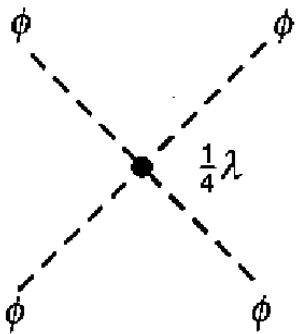
\includegraphics[width=0.2\linewidth]{higgs_boson/zelf_int_term_scal.png}
    \caption{Feynman diagram van de zelf interactie van het scalaire veld}%
    \label{fig:higgs_boson/zelf_int_term_scal}
\end{figure}

De potentiaal heeft enkel een minimum in $\phi=0$.

\begin{figure}[h]
    \centering
    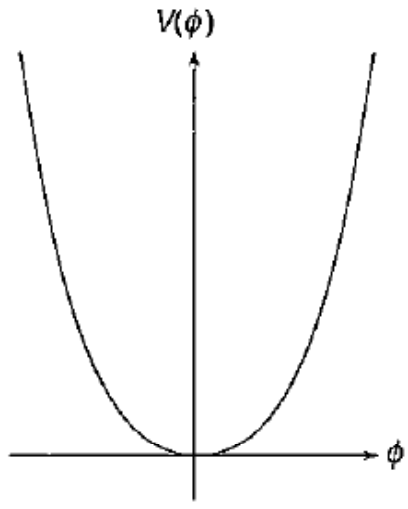
\includegraphics[width=0.2\linewidth]{higgs_boson/hoed_pot_1.png}
    \caption{De hoed potentiaal met $\mu^2>0$}%
    \label{fig:higgs_boson/hoed_pot_1}
\end{figure}

Nemen we nu $\nu^2<0$ krijgen we nu 2 minima in de potentiaal bij $\pm v$.

\begin{figure}[h]
    \centering
    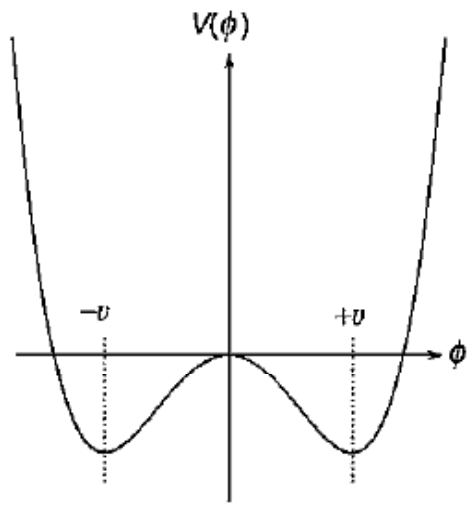
\includegraphics[width=0.2\linewidth]{higgs_boson/hoed_pot_2.png}
    \caption{De hoed potentiaal met $\mu^2<0$}%
    \label{fig:higgs_boson/hoed_pot_2}
\end{figure}

De tweede term is nu geen massaterm meer en hebben we een massaloos deeltje dat beweegt in een bepaalde potentiaal. De vacuum toestand wat de laagste toestand is ligt bij $\phi = \pm v = \pm \left| \sqrt{ \frac{-\mu^2}{\lambda}} \right|$. Dit is nu juist waar de symmetrie wordt gebroken. Nemen we nu de vacuum toestand bij $\phi = +v$ (hier maken we een verschil tussen $\pm v$ en breken we de symmetrie) is het mogelijk om $\phi$ te herschrijven.
\begin{equation}
    \begin{aligned}
        \label{eq:veld_symm_breking}
        \phi(x) &= v+\eta(x)
    \end{aligned}
\end{equation}
$eta$ is hier de beschrijving van het deeltje in de put (hoeveel deze dus afwijkt van $v$). Vullen we dit in in vergelijking (\ref{eq:lagr_hoed_pot}) geeft het volgende
\begin{equation}
    \begin{aligned}
        \label{eq:lagr_hoed_pot_symm_breking}
        \mathcal{L} &= \frac{1}{2} (\partial_\mu \eta) (\partial^\mu \eta) - \frac{1}{2} \mu^2 (v+\eta)^2 - \frac{1}{4} \lambda (v+\eta)^4\\
                    &\downarrow \mu^2= v^2\lambda\\
        &= \frac{1}{2} (\partial_\mu \eta) (\partial^\mu \eta) - \lambda v^2\eta^2 - \lambda v \eta^4 - \frac{1}{4} \lambda \eta^4 + \frac{1}{4} \lambda v^4\\
    \end{aligned}
\end{equation}
Wat we nu kunnen zien is een massief scalair veld met $m_\eta = \sqrt{2\lambda v^2}  \sqrt{-2\nu^5}$ met 2 self interacties van het $\eta$ veld.

\begin{figure}[h]
    \centering
    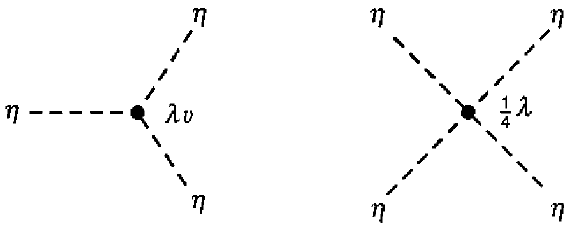
\includegraphics[width=0.4\linewidth]{higgs_boson/zelf_int_eta.png}
    \caption{Zelf interacties van het $\eta$ veld}%
    \label{fig:higgs_boson/zelf_int_eta}
\end{figure}

De laatste term in de Lagrangiaan is een constante en omdat de Lagrangiaan altijd in afgeleides voorkomt in bewegingsvergelijking is deze term niet relevant.

\subsection{Complexe scalaire velden}%
\label{sub:complexe_scalaire_velden}

Introduceren we de nu het complexe scalaire veld en de Lagrangiaan dat dat hierbij hoort.
\begin{equation}
    \begin{aligned}
        \label{eq:complex_scalair_veld}
        \phi &= \frac{1}{\sqrt{2}} (\phi_1 + i\phi_2)\\
        \mathcal{L} &= (\partial_\mu \phi)^*(\partial^\mu\phi) - \mu^2(\phi^*\phi) - \lambda(\phi^*\phi)^2
    \end{aligned}
\end{equation}
De hoed potentiaal zal in deze omstandigheden geroteerd worden rond de as loodrecht op het $\phi_1\phi_2$ vlak.

\begin{figure}[h]
    \centering
    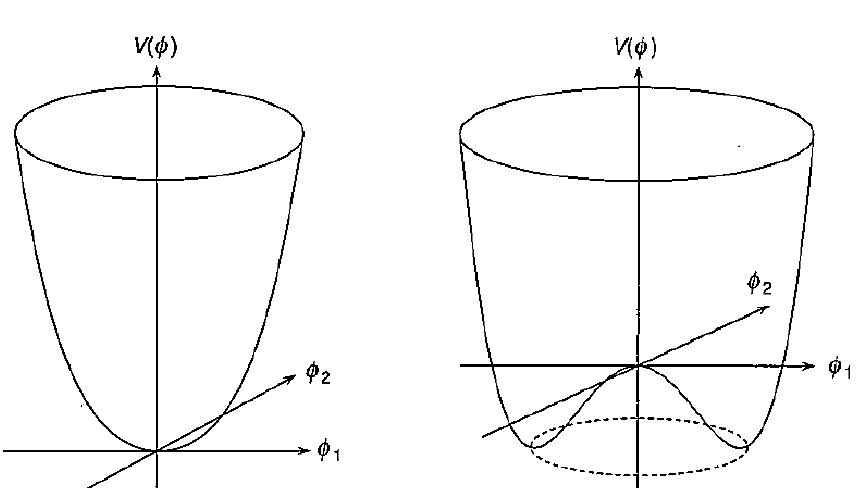
\includegraphics[width=0.6\linewidth]{higgs_boson/hoed_pot_comp.png}
    \caption{Complexe uitbreiding van de hoed potentiaal}%
    \label{fig:higgs_boson/hoed_pot_comp}
\end{figure}

Deze zal in dit geval invariant zijn onder de globale $U(1)$ transformatie $\phi \rightarrow e^{i\alpha}\phi$. Voor $\nu^2<0$ krijgen we nu een ring van minima bij
\begin{equation}
    \begin{aligned}
        \label{eq:complex_symm_breking}
        \phi_1^2+\phi_2^2 = -\frac{\mu^2}{\lambda} =v^2
    \end{aligned}
\end{equation}
We kiezen de vacuum toestand bij $(\phi_1, \phi_2) = (v,0)$ wat de globale $U(1)$ symmetrie spontaan zal breken. Expanderen we deze vacuum toestand en vullen we deze in de Lagrangiaan in dan krijgen we uiteindelijk:
\begin{equation}
    \begin{aligned}
        \label{eq:comple_scalair_veld_symm_breking}
        \phi_1(x) &= \eta(x) + v\\
        \phi_1(x) &=
    \end{aligned}
\end{equation}

\end{document}
